\documentclass{beamer}
\usepackage{amsmath}
\usetheme[numbering=fraction]{metropolis}
\usepackage[T1]{fontenc}
\usepackage{mathpazo}
\usepackage{textcomp}
\usefonttheme{professionalfonts}
\usefonttheme[onlymath]{serif}

\overfullrule=2cm

\setbeamertemplate{footline}{%
  \begin{beamercolorbox}[wd=\textwidth, sep=1ex]{footline}%
    \usebeamerfont{page number in head/foot}%
    \usebeamertemplate*{frame footer}
    \hfill%
    \usebeamertemplate*{frame numbering}
    \quad% 
  \end{beamercolorbox}%
}

% Table packages.
\usepackage{booktabs}

\usepackage{makecell}
\usepackage{tikz}

\usepackage[beamer,customcolors]{hf-tikz}
\usetikzlibrary{calc}

% This block allows to include images and bib files relative to this TeX file.
%\newcommand{\PathToTexFile}{02-presentation-v1}
%\graphicspath{\PathToTexFile}

\pdfstringdefDisableCommands{%
  \def\\{}%
  \def\texttt#1{<#1>}%
}

\setbeamercolor{background canvas}{fg=black,bg=white}

% Define useful colors.
\colorlet{black}{black!50!gray}
\colorlet{green}{green!50!gray}
\colorlet{blue}{blue!50!gray}
%\colorlet{red}{red!5}

\colorlet{CBlue}{blue!15}
\colorlet{CBlueD}{blue!50!gray}
\colorlet{CRed}{red!15}
\colorlet{CRedD}{red!50!gray}

\usepackage[protrusion,expansion,kerning,spacing,final]{microtype}

\title{Parameter estimation\\of partial differential equations\\via neural networks}
\author{Alexander Glushko, Dmitry I.\ Kabanov}
\institute{RWTH Aachen University}
\date{Final project on the Stochastic Numerics course\\Once upon a time in 2019}
\def\titlepage{%
  \usebeamertemplate{title page}%<---
}

% ------------------------------------------------------------------------------
% Useful mathematical macros
\newcommand{\Data}{\vec{D}}
\newcommand{\DataExt}{\widetilde{\vec{D}}}
\newcommand{\MSE}{\ensuremath{\text{MSE}}}
\newcommand{\T}{\ensuremath{\text{T}}}
\renewcommand{\vec}[1]{\boldsymbol{#1}}
\newcommand{\VTheta}{\ensuremath{\vec{\theta}}}
\newcommand{\VLambda}{\ensuremath{\vec{\lambda}}}
\DeclareMathOperator*{\argmin}{arg\,min}
\newcommand{\R}{\mathbb R}
\newcommand{\UNN}[1][\text{NN}]{u_{#1}}
\newcommand{\FNN}[1][\text{NN}]{f_{#1}}
\newcommand{\NonlinOp}{\mathcal N\!}
% Useful mathematical macros (end)
% ------------------------------------------------------------------------------

\begin{document}
\maketitle

% ------------------------------------------------------------------------------
% Common part
\begin{frame}{Outline}
\begin{itemize}
    \item Problem of parameter estimation of partial differential equations
          (inverse problem)
    \item How neural networks are used for the problem
    \item Intro to neural networks
    \item Example 1: linear heat equation
    \item Example~2: viscous Burger's equation
\end{itemize}
\end{frame}

%slide 2
\begin{frame}{Inverse problem}

Consider data
\[
    \vec{D} = \left\{(t_i, x_i), u_i\right\}, \quad i = 1, ..., N
\]
observed from the
model given by a partial differential equation of the form
\begin{equation*}
    \label{eq:pde}
    u_t + \mathcal N\!(u; {\color{red}\VLambda}) = 0,
\end{equation*}
with some initial and boundary conditions and \textbf{unknown} {\color{red}$\VLambda$}

{
\vspace{0.5cm}
\centering
\textbf{Goal}: estimate {\color{red}$\VLambda$}\par
}

\vspace{0.5cm}
$u=u(x, t)$ the solution of the equation (observations)\\
$\NonlinOp(u; \VLambda)$ a nonlinear algebraic-differential operator \\
$\VLambda$ the vector of unknown parameters

\end{frame}

%slide 3
\begin{frame}

The optimal $\VLambda$ found through
maximization of the posterior distribution (Bayes' rule) \cite{sivia2006data}
\begin{equation*}
    \rho( \VLambda | \Data ) \propto
    \rho( \Data | \VLambda ) \times \rho( \VLambda ).
\end{equation*}

Furthermore, we assume
\begin{align*}
    & 1)~ u_i = u(x_i, t_i; \VLambda) + \epsilon_i, \quad i=1, \dots, N, \quad \epsilon_i \sim N(0, \sigma^2),\\
    & 2) \text{ for all } \vec{\lambda} \text{ prior for } \VLambda : \quad \rho(\vec{\lambda}) = \text{const},
\end{align*}
so that, the problem of finding $\VLambda$ is a nonlinear unconstrained
optimization problem
\begin{equation*}
    \label{eq:optim-ideal}
    \argmin_{\VLambda} \quad 
    \sum_{i=1}^{N} \big[ u_i - u(x_i, t_i; \VLambda) \big]^2, 
\end{equation*}
%here noise variance $\sigma^2$ is a~
%nuisance parameter~\cite[section~8.2]{sivia2006data}
    
\end{frame}

% slide 4
\begin{frame}
% maybe include the approximate comp complexity of the analytical 
% solution
Analytical solution of the optimization problem~\eqref{eq:optim-ideal} can be expensive, so 
we replace  $u(x_i, t_i; \VLambda)$ with a 
feedforward neural network \cite{goodfellow2016deep, raissi2017pinnII}.

To ensure that $\UNN( x, t; \VTheta)$
is close to the exact solution of Eq.~\eqref{eq:pde}, we set the problem of estimating of the unknown parameters
$\VLambda$:
\begin{subequations}
\label{eq:optim-final}
\begin{align*}
    &\argmin_{\VLambda, \VTheta} \quad \ \ 
        \sum_{i=1}^N \big[u_i - \UNN(x_i, t_i; \VTheta)\big]^2  \\
    &\text{subject to } \ \ \UNN[\text{NN}, t]  + \NonlinOp(\UNN; \VLambda) = 0.
\end{align*}
\end{subequations}

\end{frame}

% slide 5
\begin{frame}
It is difficult to satisfy Eq.~\eqref{eq:optim-final} exactly as
$u_{\text{NN}}$ is an approximation of the exact solution of
Eq.~\eqref{eq:pde}.
Therefore, we relax the optimization problem introducing a NN
\begin{equation*}
    \FNN(x, t; \VLambda, \VTheta) =
        u_{\text{NN}, t} + \NonlinOp(u_{\text{NN}}; \VLambda),
\end{equation*}
where we plug the neural network $\UNN$ into Eq.~\eqref{eq:pde} and
require that $\FNN \approx 0$.

As a result, we solve the minimization problem:
\begin{equation*}
    \argmin_{\VLambda, \VTheta}
    \sum_{i=1}^N \big[ u_i - \UNN(x_i, t_i; \VTheta)\big ]^2
    +\gamma \sum_{i=1}^N \big[ \FNN(x_i, t_i; \VLambda, \VTheta) \big]^2,
\end{equation*}
here $\gamma$ is a regularization hyperparameter that is chosen via cross-validation.
    
\end{frame}

%slide 6
\begin{frame}{Description of neural networks}
    
Let us recall the neural network equation:
$$
\UNN(x, t; \vec{\theta}) = g_L \circ g_{L-1} \circ \dots \circ g_1,
$$
where
\[
    g_\ell(z; \VTheta_\ell) = \sigma (W_\ell z + b_\ell), \quad \ell = 1,\dots,L.
\]
Here 
\begin{itemize}
    \item $L$  - is the number of layers in the network,
    \item 0s layer and $L$th layer are input and output layers, respectively,
    \item layers from 1 to $L-1$ - are hidden layers,
    \item $\sigma = \tanh (z) $ - is a nonlinear activation function applied componentwise.
\end{itemize} 
 
The neural-network parameter $\VTheta$ contains the components of matrices
$W_\ell \in \R^{n_{\ell}\times n_{\ell-1}}$ and bias vectors
$b_\ell \in \R^{n_\ell}$, where $n_\ell$  (number of "neurons") denotes the width of the
$\ell$\textsuperscript{th} layer.
    
\end{frame}

% slide 7
\begin{frame}

Below, one can see the general scheme of the neural network:
\begin{figure}
\centering
\label{fig:network}
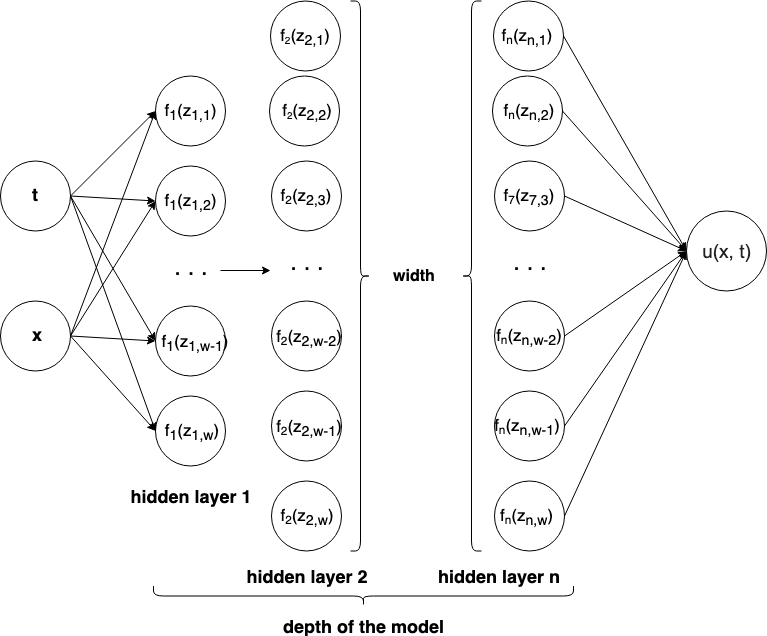
\includegraphics[width = 10cm , height = 7cm]{images/FFNN.png}
\\
\caption{Feed forward neural network.}
\end{figure}
\end{frame}

\begin{frame}{Why neural network is better than solving full PDE problem?}
Neural network must be evaluated only at the observation points\\
PDE problem must be computed on a grid, which includes observation points as a subset
\end{frame}

\begin{frame}{Neural network computational complexity}
    Let us denote $n^{(k)}$ the number of neurons in the $k$th layer, $L$ as the number of layers. Then the number of multiplications of weights is: $$n_{mul} = \sum_{k=2}^{L} n^{(k)}n^{(k-1)}n^{(k-2)} + n^{(1)}n^{(0)}*2.$$
    The number of activation function use is: $$n_g = \sum_{k = 1}^{L} n^{(k)}.$$ Therefore, $ \text{ the computational complexity is } = n_{mul} + n_g = O(n^4) + O(n^2) \Longleftrightarrow O(n^4).$ 
\end{frame}

\begin{frame}{Hyperparameter $\gamma$ is chosen via $K$-fold cross-validation}
\begin{equation*}
    \argmin_{\VLambda, \VTheta}
    \sum_{i=1}^N \big[ u_i - \UNN(x_i, t_i; \VTheta)\big ]^2 \enspace + \enspace
    \tikzmarkin<1>[set fill color=CBlue, set border color=CBlueD]{gamma}\gamma
    \tikzmarkend{gamma}
    \,
    \sum_{i=1}^N \big[ \FNN(x_i, t_i; \VLambda, \VTheta) \big]^2,
\end{equation*}
\vspace{0.5cm}

In a usual case, regularization parameter is used to "punish" big values of a model parameters $\vec{\theta}$, that lead to the overfitting, of the neural network. In our case, we use it as a constraint for the model. 

\end{frame}

\begin{frame}{Cross-validation (CV) algorithm}
    We use CV in order to validate the regularization hyperparameter $\vec{\gamma}$.\\
    \vspace{0.5cm}
    1) split the observed data $\vec{D} = \left\{(t_i, x_i), u_i\right\}, \quad i = 1, ..., N$ into $k = 5$ folds.\\
    \vspace{0.5cm}
    2) Repeat k times for a chosen $\gamma$ value: \\
        \quad - train the neural network on $k - 1$ folds\\
        \quad - test on the left part\\
        \quad - average the results over all $k$ folds.\\
    \vspace{0.5cm}
    3) Choose the result with the least MSE.
\end{frame}

\begin{frame}{Bootstrapping parameters $\vec{\lambda}$}
    In this work, model parameter $\vec{\lambda}$ is estimated using bootstrap technique:\\
    \vspace{0.5cm}
    \quad - Set training and test data.\\
    Repeat for a several times $T$ the following steps:\\
    \quad - Choose 80\% of the sample data and use it for training and testing the model. \\
    \quad - Store the resulting $\vec{\lambda}$.\\
    \vspace{0.5cm}
    Results of bootstrap are given below for each problem.
\end{frame}

% Common part (end)
% ------------------------------------------------------------------------------


% ------------------------------------------------------------------------------
% Heat equation part

\section{Example 1. Heat equation}

\begin{frame}{Heat equation}
We consider the linear heat equation
\begin{align*}
    &u_t - {\color{red}\lambda} u_{xx} - g(x, t) = 0, \quad x\in[-1; 1], \quad t\in[0, 1] \\
    &u(x, 0) = 0 \\
    &u(0, t) = u(1, t) = 0
\end{align*}
with source term $g(x, t) = (4\pi^2 -1) \, \sin(2\pi x) \, \exp(-t)$

\vspace{0.5cm}
True $\lambda$ is 1

Exact solution: $\quad u = \sin(2\pi x) \, \exp(-t)$
\end{frame}

\begin{frame}{Observations}
1. Compute $u$ on the uniform grid with $201\times101$ points in $x\times t$\\
2. Network complexity [2, 20, 20, 1]: 2 hidden layers with 20 neurons in each\\
3. In total $2\times20 + 20 + 20\times20 + 20 + 20\times1+1=501$ parameters in $\VTheta$\\
4. Sample 6400 observations uniformly\\
5. Large number of observations allows to avoid overfitting.
\end{frame}

\begin{frame}{Observations}

\centering
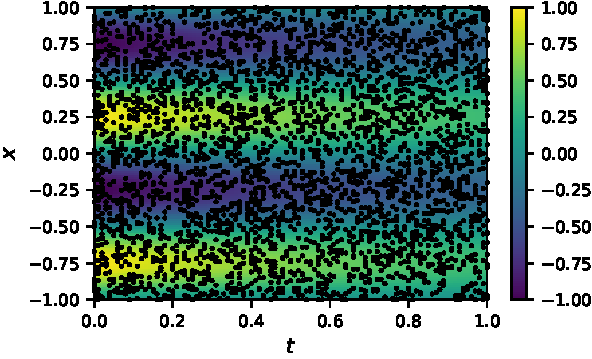
\includegraphics{images/heateq-observations}
\end{frame}

\begin{frame}{Cross-validation for $\gamma$}
\centering
Clean data: just exact solution

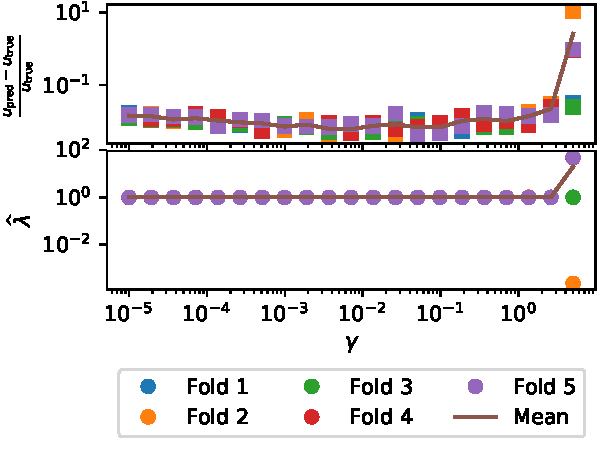
\includegraphics{images/heateq-cross-validation}
\end{frame}

\begin{frame}{Cross-validation for $\gamma$}
\centering
Noisy data: $\quad u_{\text{obs}} = u +  N(0, \sigma^2), \quad \sigma=0.05 \sqrt{u}$

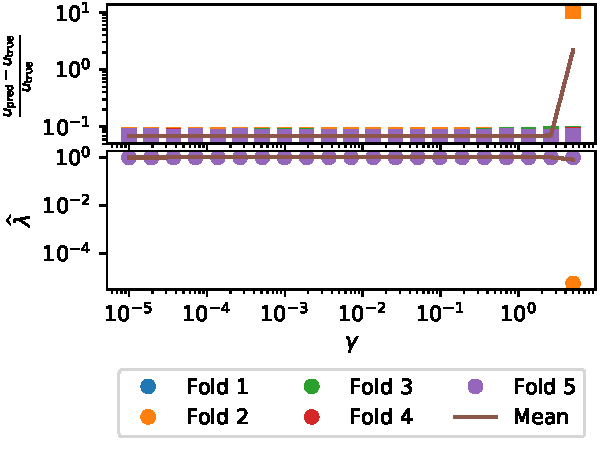
\includegraphics{images/heateq-cross-validation-with-noise}
\end{frame}


\begin{frame}{Cross-validation for $\gamma$}
    For given neural network, results are insensitive to the value of $\gamma$
    for $\gamma$ less than $\approx 2$\\
    At least for the present problem

\end{frame}

\begin{frame}{Bootstrap}
Still computing... To be finished
\end{frame}

\begin{frame}{Preliminary results with $\gamma=2$}
Training the network with $\gamma=2$ gives prediction $\widehat{\lambda} =
1.00175$ with error $\approx 0.18 \,\%$.

\vspace{0.5cm}
\centering
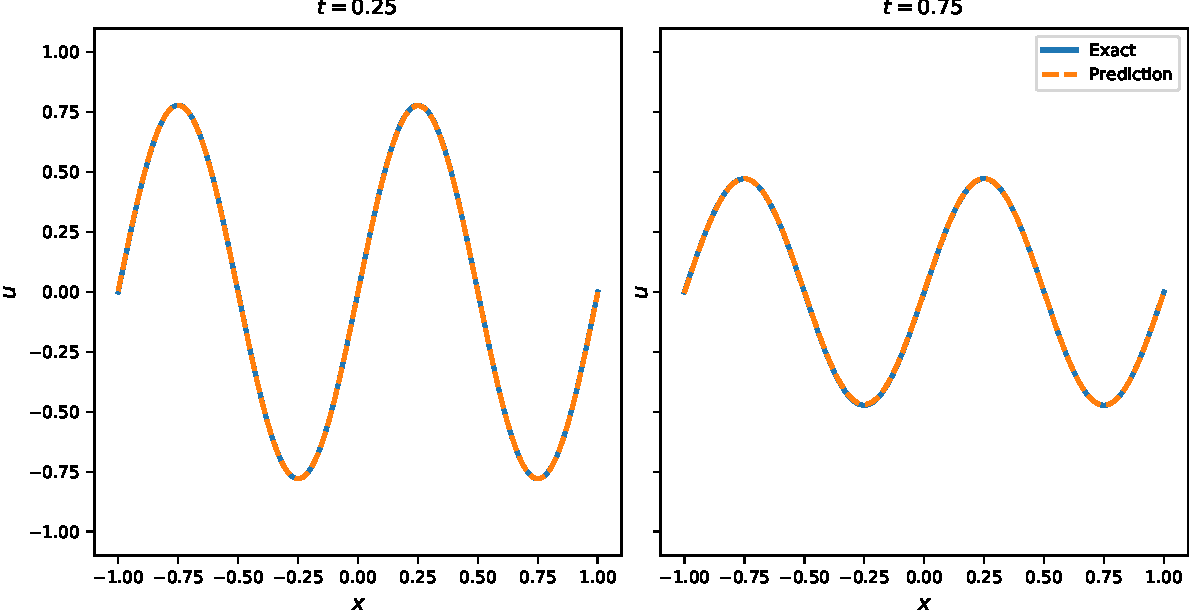
\includegraphics[scale=0.55]{images/heateq-predictions}

\end{frame}

% Heat equation part (end)
% ------------------------------------------------------------------------------


% ------------------------------------------------------------------------------
% Burgers' equation

\section{Example 2. Burgers' equation}

\begin{frame}{Burgers' equation}
We consider the input data of the Burgers' equation:
\begin{align*}
&u_t + \lambda_1 u u_x - \lambda_2 u_{xx} = 0, \quad x\in[-1, 1], \quad t\in[0, T]\\
&u(0, x) = -\sin(\pi x) \\
&u(t, -1) = u(t, 1) = 0
\end{align*}

with true values of the sought-for parameters
\[
    \lambda_1 = 1,  \quad \lambda_2 = (0.01 / \pi) \approx 0.318.
\]

The exact solution is
$$u(t, x) = \frac{\pi \lambda_2}{\pi \lambda_2 e^{\{\pi^2 \lambda_2 t\}} - (e^{\{\pi^2 \lambda_2 t\}} - 1) cos(\pi x)}$$

\end{frame}

\begin{frame}{Burgers' equation neural network configuration}
    For this problem 3200 observations were used. The optimal number of them is: $2*M^2$, where $M$ is the number of model parameters. As we have 4 hidden layers with 10 neurons in each. This number basically affects the underfitting and overfitting of the neural network. \\
    
    The computational complexity according to the configuration of an NN consists of the number of matrix multiplications and the amount of the activation function use. 
    
\end{frame}

\begin{frame}{Observations}
\small
Below, the exact solution is depicted on the uniform grid with 201 points in $x$ and 101 points in $t$. 
\begin{figure}
    \centering
    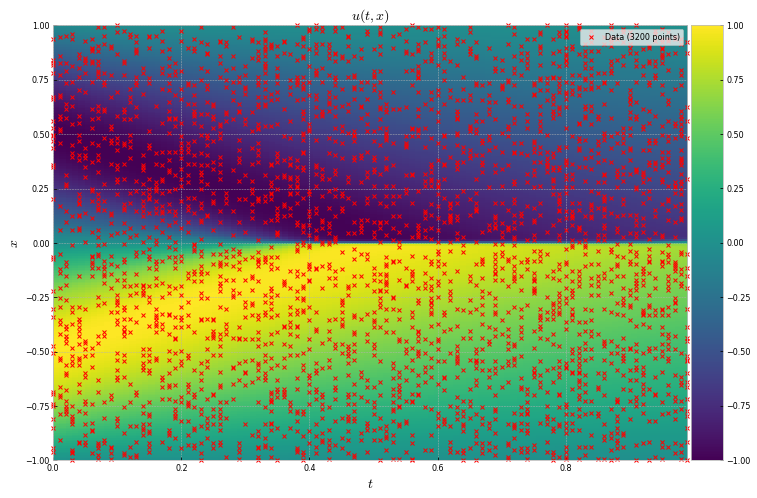
\includegraphics[width=10cm, height=6cm]{images/burgers-exact.png}
    \caption{The exact solution of Burgers' equation and 3200 observations.}
    \label{fig:my_label}
\end{figure}

\end{frame}

\begin{frame}

Hyperparameter $\gamma$ for the optimization problem was computed via cross-validation technique, using 5 folds. 
\begin{figure}
    \centering
    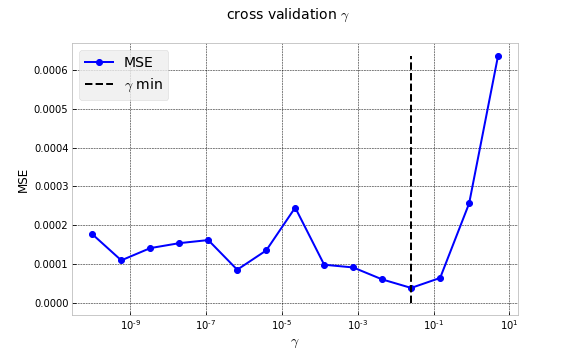
\includegraphics[width=11cm, height=6cm]{images/burgers-cross_val_gamma.png}
    \caption{Cross-validation result for the hyperparameter $\gamma = 0.0255$.}
    \label{fig:cross_val_gamma}
\end{figure}

\end{frame}

\begin{frame}

Hyperparameter $\gamma$ for noisy data: $u_{obs} = u + N(0, \sigma^2),$ $\sigma = 0.05\sqrt{u}.$ 

\begin{figure}
    \centering
    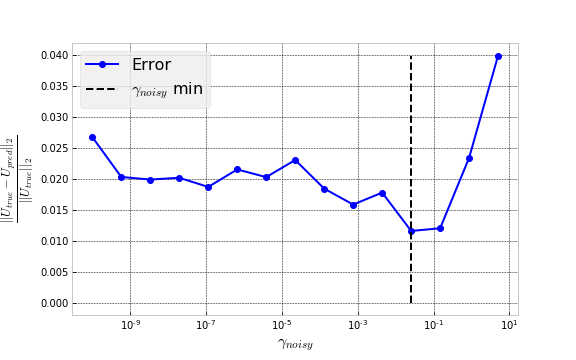
\includegraphics[width=11cm, height=6cm]{images/burgers-cross_val_gamma_noisy.png}
    \caption{Cross-validation result for the hyperparameter $\gamma = 0.0255$ on the noisy data.}
    \label{fig:cross_val_gamma_noisy}
\end{figure}
    
\end{frame}

\begin{frame}{Results with $\gamma=0.02553$}
Below, we present a comparison between the exact and the predicted solutions at the different time instants t = 0.25, 0.50, 0.75. Training the network with $\gamma=0.0255$ gives prediction $\lambda_1 =
0.986564, ~ \lambda_2 = 0.00338$ with MSE $u(x, t) \approx 0.011 \,\%$.

\begin{figure}
    \centering
    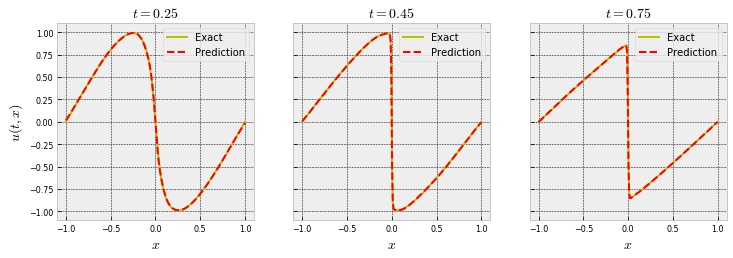
\includegraphics[scale=0.43]{images/burgers-exact-predict.png}
    \caption{The exact and predicted solutions of Burgers' equation in time.}
    \label{fig:burgers-exact-predict}
\end{figure}

\end{frame}

\begin{frame}{}

We have got the following bootstrapped results:
\begin{figure}
\centering
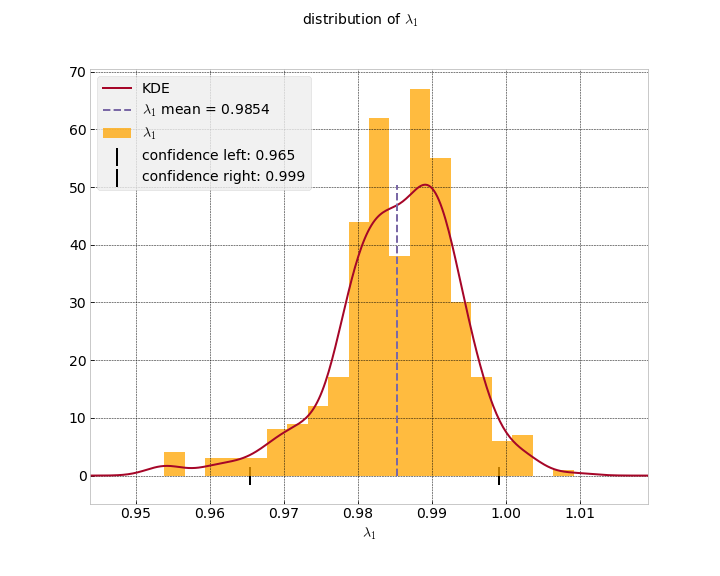
\includegraphics[width = 9cm , height = 7cm]{images/burgers-bootstraped_l1.png}
\caption{Bootstrapped parameter $\lambda_1$ for Burgers' equation.}
\end{figure}

\end{frame}

\begin{frame}

\begin{figure}
    \centering
    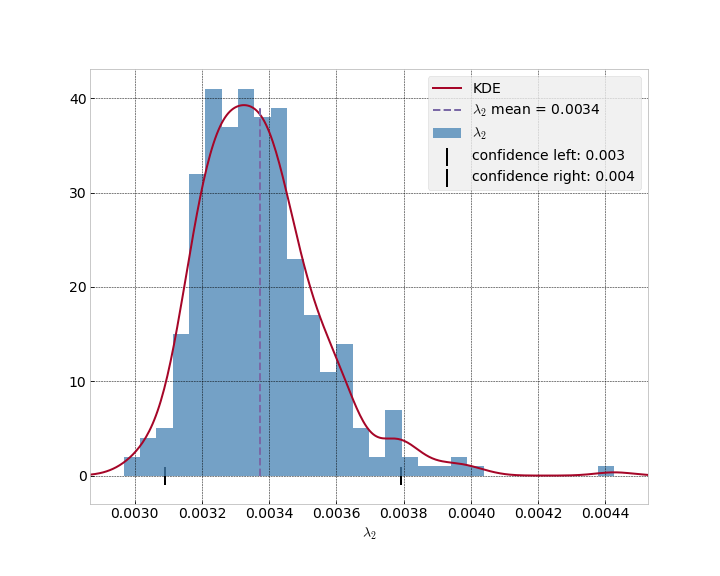
\includegraphics[width = 10cm , height = 8cm]{images/burgers-bootstraped_l2.png}
    \caption{Bootstrapped parameter $\lambda_2$ for Burgers' equation.}
    \label{fig:bootstraped_l2}
\end{figure}
    
    
\end{frame}

\begin{frame}{Neural Network configuration vs $\lambda$ error}

Below one can see the \% error in $\lambda_1$ and $\lambda_2$ for different neural network configurations. In the first column the number of the hidden layers is presented, in the second row the number of the neurons in each hidden layer is presented.

\begin{tabular}{lccc|ccc}
    \toprule
    & \multicolumn{3}{c}{\% error in $\lambda_1$} & \multicolumn{3}{c}{\% error in $\lambda_2$}\\
  \midrule
%  \diagcell{.2em}{1.4cm}{\tiny{Layers}}{\tiny{Neurons}}
\diaghead{Columnmnm}{Layers}{Neurons} & 5 & 10 & 20 & 5 & 10 & 20 \\
\midrule
  1 & 19.43 & 31.82 & 25.32 & 118.02 & 79.2 & 74.33\\
  \hline
  2 & 24.93 & 8.75 & 3.21 & 56.05 & 28.35 & 23.48\\
  \hline
  4 & 3.42 & 0.82 & 0.29 & 13.56 & 2.43 & 4.21\\
  \hline
  6 & 3.26 & 2.16 & 1.29 & 19.53 & 2.79 & 0.66\\
  \hline
  8 & 6.17 & 1.41 & 2.83 & 6.57 & 1.26 & 1.28\\
  \bottomrule
\end{tabular}

\end{frame}

\begin{frame}{Neural Network vs predicted solution error}

Below one can see the \% error in solution for different neural network configurations. 

\centering
    \begin{tabular}{lccc}
    \toprule
    & \multicolumn{3}{c}{\% error in solution $u(x, t)$} \\
    \midrule
    \diaghead{Columnmnm}{Layers}{Neurons}& 5 & 10 & 20  \\
    \hline
    1 & 0.191595 & 0.159833 & 0.134457 \\
    \hline
    2 & 0.069515 & 0.029497 & 0.021157 \\
    \hline
    4 & 0.015328 & 0.010501 & 0.007361 \\
    \hline
    6 & 0.020529 & 0.010405 & 0.005556 \\
    \hline
    8 & 0.026048 & 0.008358 & 0.009048 \\
    \bottomrule
    \end{tabular}
    
    From the results above one can see that the optimal configuration of the model is: 6 hidden layers with 20 neurons in each.
\end{frame}

% Burgers' equation (end)
% ------------------------------------------------------------------------------

\begin{frame}
    \frametitle{Conclusions}
    
Therefore, a key property of physics informed neural networks is that they can be effectively trained using small data sets; a setting often encountered in the study of physical systems for which the cost of data acquisition may be prohibitive.

\end{frame}


\bibliography{presentation}
\bibliographystyle{abbrv}

\end{document}
